\documentclass[xcolor=dvipsnames,12pt,aspectratio=169]{beamer}
\usecolortheme[named=violet]{structure} 

%\usetheme{umbc2} 
\usepackage{pgf}
%\usepackage[pdftex]{graphicx}
\usepackage{color}
\usepackage{amssymb,amsmath}
\usepackage[english]{babel}
\mode<presentation>

 \usepackage{multimedia}
\usefonttheme{structurebold}

%\useinnertheme{umbcboxes}

%\setbeamercolor{umbcboxes}{bg=violet!15,fg=black}  

\setbeamercovered{transparent}
\setbeamertemplate{navigation symbols}{}

%
%
% Adjustable parenthesis et al
%
\newcommand{\K}[1]{\left({#1}\right)}
\newcommand{\lp}{\left(}
\newcommand{\rp}{\right)}
\newcommand{\lb}{\left[}
\newcommand{\rb}{\right]}
\newcommand{\lc}{\left\{}
\newcommand{\rc}{\right\}}
\newcommand{\la}{\left\langle}
\newcommand{\ra}{\right\rangle}
\newcommand{\Dp}[3]{\langle #1,#2 \rangle_{#3}}
\newcommand{\cov}[2]{\langle #1\,#2 \rangle}

\newcommand{\half}{\mbox{$\frac{1}{2}$}} %

\newcommand{\U}{{\cal U}}
\newcommand{\C}{{\cal C}}
\newcommand{\X}{{\cal X}}
\newcommand{\Y}{{\cal Y}}

\newcommand {\ared} {{\rm ared}}
\newcommand {\pred} {{\rm pred}}
\newcommand {\rpred} {{\rm rpred}}

\newcommand{\sn}{s^{\sf n}}  % Normal component
\newcommand{\st}{s^{\sf t}}  % Tangential component
\newcommand{\rt}{r^{\sf t}}  % Tangential component
\newcommand{\stepy}{{s_y}}  % step in y--component
\newcommand{\stepu}{{s_u}}  % step in u--component

%
\newcommand{\veps}{{\varepsilon}} 
% Bolds and scripts
%
\newcommand{\CG}{\ensuremath{\mathcal{G}} }
\newcommand{\CQ}{\ensuremath{\mathcal{Q}} } %
\newcommand{\CR}{\ensuremath{\mathcal{R}} } %
\newcommand{\CW}{\ensuremath{\mathcal{W}} } %
\newcommand{\CX}{\ensuremath{\mathcal{X}} } %
\newcommand{\CZ}{\ensuremath{\mathcal{Z}} } %
\newcommand{\CU}{\ensuremath{\mathcal U} }
\newcommand{\CC}{\ensuremath{\mathcal C} }
\newcommand{\CD}{\ensuremath{\mathcal D} }
\newcommand{\BA}{\ensuremath{\mathbf{A}} } %
\newcommand{\BB}{\ensuremath{\mathbf{B}} } %
\newcommand{\BC}{\ensuremath{\mathbf{C}} } %
\newcommand{\BhC}{\ensuremath{\widehat{\mathbf{C}}} } %
\newcommand{\BD}{\ensuremath{\mathbf{D}} } %
\newcommand{\BE}{\ensuremath{\mathbf{E}} } %
\newcommand{\BF}{\ensuremath{\mathbf{F}} } %
\newcommand{\BG}{\ensuremath{\mathbf{G}} } %
\newcommand{\BH}{\ensuremath{\mathbf{H}} } %
\newcommand{\BK}{\ensuremath{\mathbf{K}} } %
\newcommand{\BL}{\ensuremath{\mathbf{L}} } %
\newcommand{\BM}{\ensuremath{\mathbf{M}} } %
\newcommand{\BN}{\ensuremath{\mathbf{N}} } %
\newcommand{\BP}{\ensuremath{\mathbf{P}} } %
\newcommand{\BQ}{\ensuremath{\mathbf{Q}} } %
\newcommand{\BR}{\ensuremath{\mathbf{R}} } %
\newcommand{\BU}{\ensuremath{\mathbf{U}} } %
\newcommand{\BW}{\ensuremath{\mathbf{W}} } %
\newcommand{\BX}{\ensuremath{\mathbf{X}} } %
\newcommand{\BY}{\ensuremath{\mathbf{Y}} } %
\newcommand{\BZ}{\ensuremath{\mathbf{Z}} } %
\newcommand{\ba}{\ensuremath{\mathbf{a}}}
\newcommand{\bb}{\ensuremath{\mathbf{b}}}
\newcommand{\bc}{\ensuremath{\mathbf{c}}}
\newcommand{\be}{\ensuremath{\mathbf{e}}}
\newcommand{\bg}{\ensuremath{\mathbf{g}}} %
\newcommand{\bh}{\ensuremath{\mathbf{h}}} %
\newcommand{\bk}{\ensuremath{\mathbf{k}}} %
\newcommand{\bn}{\ensuremath{\mathbf{n}}} %
\newcommand{\bp}{\ensuremath{\mathbf{p}}} %
\newcommand{\bq}{\ensuremath{\mathbf{q}}}
\newcommand{\br}{\ensuremath{\mathbf{r}}} %
\newcommand{\bs}{\ensuremath{\mathbf{s}}} %
\newcommand{\bt}{\ensuremath{\mathbf{t}}} %
\newcommand{\bu}{\ensuremath{\mathbf{u}}} %
\newcommand{\bv}{\ensuremath{\mathbf{v}}} %
\newcommand{\bdv}{\ensuremath{\mathbf{\delta v}}} %
\newcommand{\bw}{\ensuremath{\mathbf{w}}} %
\newcommand{\bd}{\ensuremath{\mathbf{d}}} %
\newcommand{\bx}{\ensuremath{\mathbf{x}}} %
\newcommand{\by}{\ensuremath{\mathbf{y}}} %
\newcommand{\obx}{\ensuremath{\overline{\mathbf{x}}}} %
\newcommand{\oby}{\ensuremath{\overline{\mathbf{y}}}} %
\newcommand{\obz}{\ensuremath{\overline{\mathbf{z}}}} %
\newcommand{\obw}{\ensuremath{\overline{\mathbf{w}}}} %
\newcommand{\bz}{\ensuremath{\mathbf{z}}} %
\newcommand{\blambda}{\mbox{\boldmath $\lambda$}}
\newcommand{\bdelta}{\mbox{\boldmath $\delta$}}
\newcommand{\bxi}{\mbox{\boldmath{$\xi$}}}
\newcommand{\bfeta}{\mbox{\boldmath $\eta$}}
\newcommand{\bkappa}{\mbox{\boldmath $\kappa$}}
\newcommand{\bmu}{\mbox{\boldmath $\mu$}}
\newcommand{\brho}{\mbox{\boldmath $\rho$}}
\newcommand{\bsigma}{\mbox{\boldmath $\sigma$}}
\newcommand{\sbxi}{\mbox{\scriptsize \boldmath{$\xi$}}}
\newcommand{\sbfeta}{\mbox{\scriptsize \boldmath $\eta$}}
\newcommand{\teta}{\mbox{\tiny \boldmath $\eta$}}
\newcommand{\txi}{\mbox{\tiny \boldmath{$\xi$}}}
\newcommand{\bLambda}{\mbox{\boldmath $\Lambda$}}
\newcommand{\bDelta}{\mbox{\boldmath $\Delta$}}
\newcommand{\bzero}{\mbox{\boldmath $0$}}
\newcommand{\bone}{\mbox{\boldmath $1$}}
\newcommand{\sDelta}{\mbox{\small $\Delta$}}
\newcommand{\tDelta}{\mbox{\tiny $\Delta$}}

\newcommand{\pd}[2]{\frac{\partial #1}{\partial #2}}
\newcommand{\ppd}[3]{\frac{\partial^{#3} #1}{\partial {#2}^{#3}}}
\newcommand{\pdsec}[3]{\frac{\partial^2 #1}{\partial #2\partial #3}}

\def\frechet{Fr\'echet\ }
%\newcommand{\real}{\mathbb{R}}
\newcommand{\real} {I\!\!R}
\newcommand{\nat} {{I\!\!N}}
\newcommand{\compl} {C\!\!\!\!I\;}
%
\def\Pr{\sf Pr}
\def\Re{\sf Re}
\def\M{{\sf M}}
\def\d{\delta}
\newcommand{\deq}{\raisebox{0pt}[1ex][0pt]{$\stackrel{\scriptscriptstyle{\rm def}}{{}={}}$}}
\newcommand{\dif}{{\mathrm d}}

\newcommand{\eref}[1]{\mbox{\rm(\ref{#1})}}
\newcommand{\tref}[1]{\mbox{\rm\ref{#1}}}


%\newenvironment{proof}{\noindent {\bf Proof:} }{\hfill $\Box$ \\[2ex] }

\newcommand{\myint}[1]{\int_0^T \dif t~{#1}}
\newcommand{\myintt}[1]{\int_0^1 \dif s~{#1}}
\newcommand{\dint}[1]{\int\limits_{#1}\!\!\!\int}

\newcommand{\waveop}[1]{c^{-2}{#1}_{tt}-\Delta{#1}}
\newcommand{\redwaveop}[1]{\Delta{#1}+k^2n^2{#1}}

\newcommand{\D}{\displaystyle}
%\allowdisplaybreaks
%

\setlength{\parskip}{2ex}   % place a blank line between paragraphs
\def\Logo{\@ifnextchar(\beamer@Logo\logo}
\def\beamer@Logo(#1,#2){\logo}

\AtBeginSection[]{
{\setbeamertemplate{logo}{}
 \begin{frame}<beamer>
    \frametitle{Agenda}
    \tableofcontents[currentsection]
  \end{frame}
}
}
% Images
% Macros
\newcommand{\peq}{\,+\hspace{-0.15cm}=}
\newcommand{\bm}{\bar{m}}
\newcommand{\dm}{\delta m}
\newcommand{\dom}{\delta \bar{m}}
\newcommand{\doma}{\delta \bar{m}_{\alpha}}
\newcommand{\om}{\bar{m}}
\newcommand{\bH}{{\bf H}}
\newcommand{\bR}{{\bf R}}
\newcommand{\bcF}{{\bar{\cal F}}}
\newcommand{\cF}{{\cal F}}
\newcommand{\oF}{\bar{F}}
\newcommand{\odF}{\bar{F}^{\dagger}}
\newcommand{\oS}{\bar{S}}
\newcommand{\oM}{\bar{M}}
\newcommand{\Ja}{J_{\alpha}}
\newcommand{\Na}{N_{\alpha}}
\newcommand{\dd}{\delta d}
\newcommand{\ddl}{\delta d_{\alpha}}


\title[]{Extended Inversion: when it works, and why}
\author[]{William W. Symes}
\institute[]{symes@rice.edu}
\date{December 2020}

\begin{document}
\frame{
\titlepage
}

\begin{frame}\frametitle{Overview}
Apply sophisticated methods to a simple inversion problem

Why:
\begin{itemize}
\item clear understanding of what works and what doesn't, and why
\item all details ``on paper''
\item conclusions not justified only ``in rear view mirror'' by a few numerical examples
\item road map for application to industrially relevant technology
\end{itemize}

{\em ``You can do this at home!''}

Thanks to Prof. Sue Minkoff and GRA Huiyi Chen, UT Dallas
\end{frame}

\begin{frame}\frametitle{World's simplest waveform inversion problem}
\only<1>{
Single trace transmission in a fluid:

Point source at $\bx=\bx_s$ radiates with transient intensity $w(t)$ (``wavelet'')

Resulting pressure wave propagates to point receiver at $\bx=\bx_r$, offset $|\bx_r-\bx_s|=h$

Pressure trace predicted by linear acoustics:
\[
p(t) = \frac{1}{4\pi h}w(t-mh) = (F[m]w)(t)
\]
where $m =$ pressure wave slowness ($=1/v_p$), $F$ = modeling operator - linear in w, nonlinear in $m$
}
\only<2>{
Inverse problem: given pressure trace $d(t)$, wavelet $w(t)$, and offset $h$, find slowness $m$ so that
\[
F[m] w  \approx d
\]
Can solve by inspection! Use a ruler to measure time shift between $w(t)$ and $w(t-mh)$

BUT let's use the standard approach instead: turn it into an optimization - minimize over $m$ the {\em mean square error}
\[
\frac{1}{2}\int\,dt\, (F[m]w(t) -d(t))^2 = \frac{1}{2}\|F[m]w-d\|^2 = J_{\rm FWI}[m;w,d]
\]
= world's simplest FWI task
}
\end{frame}

\begin{frame}\frametitle{How to cycle-skip, in one easy lesson}
\only<1>{
Asymptotic transient-ness:

Mother wavelet $w_1$: $w_1(t)=0, |t|>1$ and $\int w_1^2 = 1$

Scaled wavelets $w_{\lambda} = \frac{1}{\sqrt{\lambda}}w_1(t/\lambda)$: $w_{\lambda}(t)=0, |t|>\lambda$ and $\int w_{\lambda}^2 = 1$

NB: if center frequency of $w_1 = \omega_1$, then center frequency of $w_{\lambda} = \omega_1/\lambda$
}
\only<2>{

Theorem Uh-Oh: If $d = F[m_*]w_{\lambda}$ (noise-free transient data) and $|m-m_*| > 2\lambda/h$, then
\[
J_{\rm FWI}[m;w_{\lambda},d] = \|d\|^2, \,\, \nabla_m J_{\rm FWI}[m;w_{\lambda},d] = 0
\]
Proof.
\begin{center}
\vspace{-0.5cm}
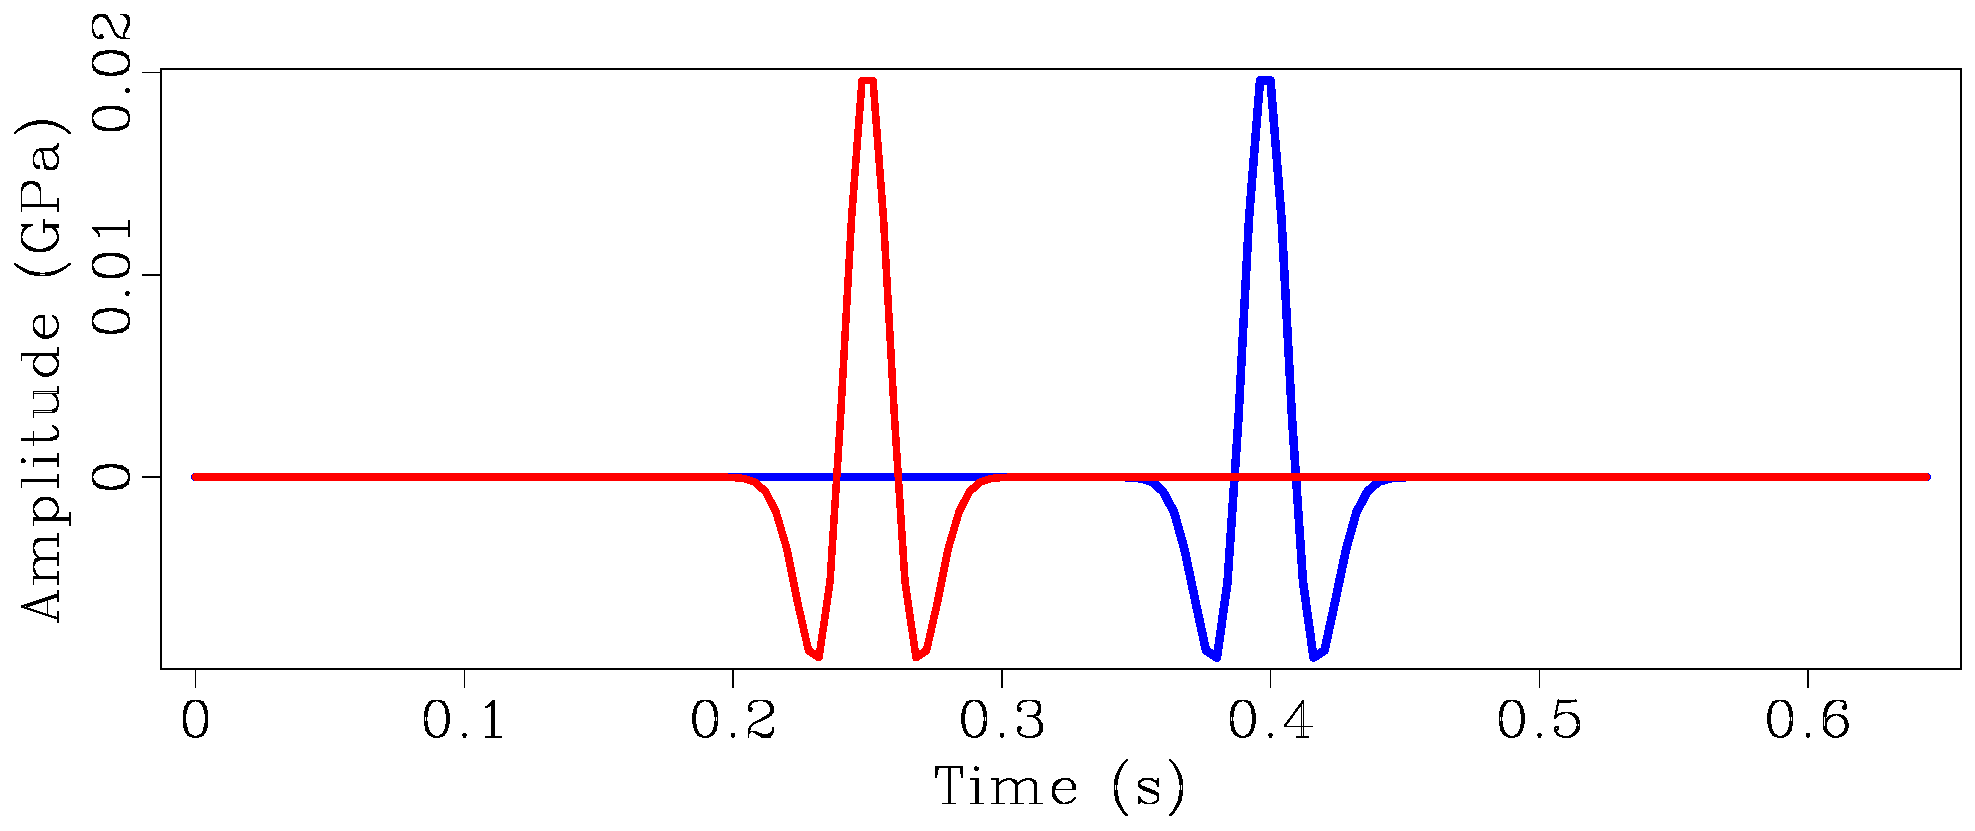
\includegraphics[height=3cm]{Fig/datas.pdf}\\
Data: same wavelet, $m$ = 0.25 s/km (red) and $m_*$ = 0.4 s/km (blue)
\end{center}
\vspace{-0.5cm}
$F[m]w_{\lambda}$ orthogonal to $F[m_*]w_{\lambda}$ if $|m-m_*| > 2\lambda/h$
\hfill Q. E. D.
}
\only<3>{
$J_{\rm FWI}$: $d=F[m_*]w_{\lambda}$, $m_*=0.4$ s/km, $w_{\lambda}$ = Ricker ctr freq = $1/\lambda$ Hz, $h=1$ km
\vspace{-0.5cm}
\begin{center}
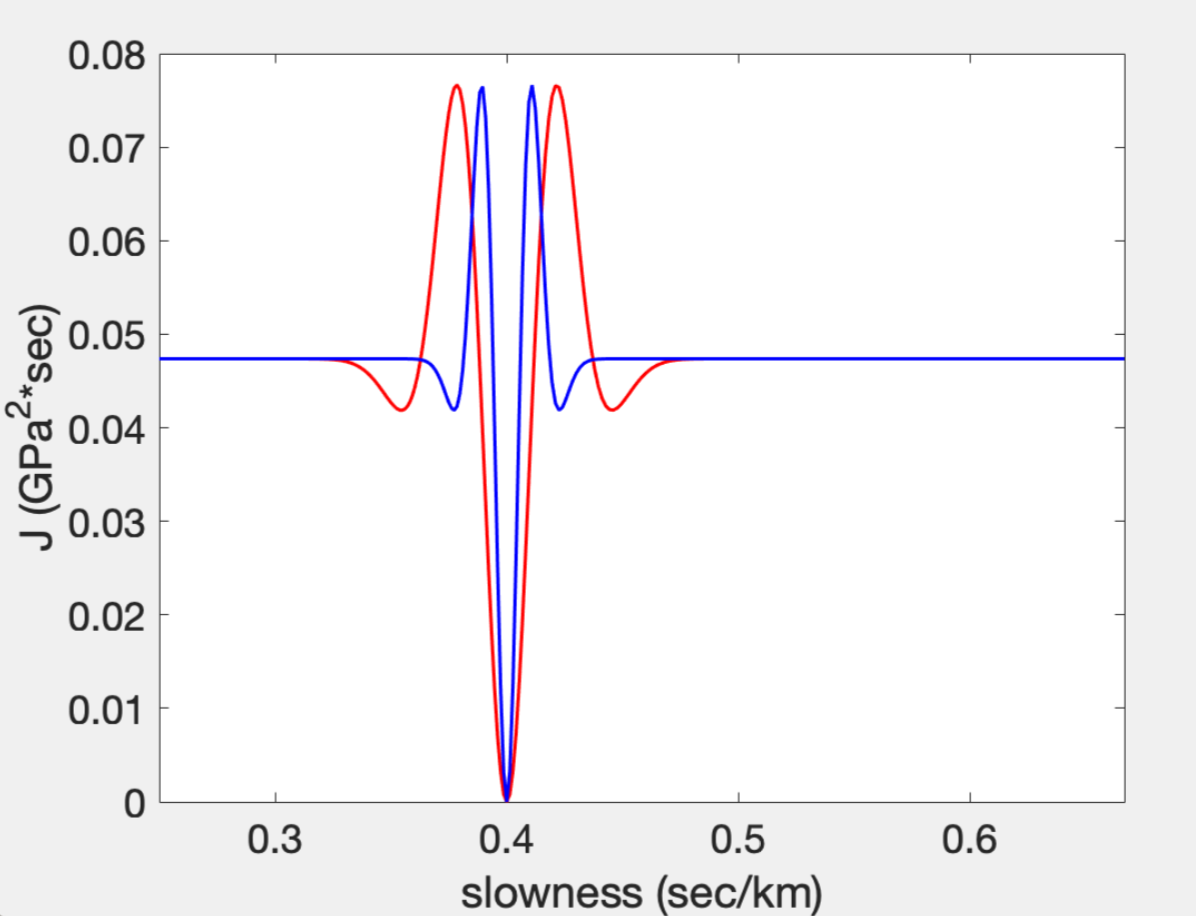
\includegraphics[height=5cm]{Fig/FWI.png}
\end{center}
\vspace{-0.5cm}
Red: $\lambda=0.05$ s (20 Hz), Blue: $\lambda = 0.025$ s (40 Hz) [H. Chen et al. SEG 20]
}
\only<4>{
Postmortem:

\begin{itemize}
\item for most $m$, predicted data $F[m]w$ is not close to target data $d$
\item for most $m$, gradient is not a useful search direction
\item shape of objective function depends strongly on data frequency content - large residual, useless gradient more common for high frequencies (small $\lambda$)
\item flip side: low frequency (big $\lambda$) $\Rightarrow$ useful updates for larger set of initial models
\end{itemize}
}
\end{frame}

\begin{frame}\frametitle{Wavefield Reconstruction Inversion}
\only<1>{
Extended inversion: {\em enlarge the model space} = add (nonphysical) degrees of freedom, converge to point in original model space

Rationale: more likely to be able to 
\begin{itemize}
\item find low residual (extended) models (``hug your data''),
\item explore useful update directions
\end{itemize}

WRI - van Leeuwen \& Herrmann GJI 13, IP 16, many other papers - most studied extended inversion approach

Idea: view wave equation as {\em weak constraint} $\sim$ {\em add source parameters}

}
\only<2>{
Cast: 
\begin{itemize}
\item model parameters $m$ (eg. $m$=slowness)
\item Wave operator $L[m]$ (eg. constant density acoustic op $L[m]=m^2\partial_t^2 - \nabla^2$)
\item Known (!) source field $q(\bx,t)$ (eg. point source $w(t)\delta(\bx-\bx_s)$)
\item dynamic fields $u(\bx,t)$ solve $L[m]u=q$ (eg. $u=$ pressure)
\item Sampling operator $P$ extracts data trace(s) (pressure or ...) from $u$
\item Modeling operator $F[m]=PL[m]^{-1}$
\end{itemize}
}
\only<3>{
FWI: given $d$, $q$, 
\[
\min_m \|Pu-d\|^2 \mbox{ subj to } L[m]u=q
\]
\[
\Leftrightarrow \min_m \|F[m]q-d\|^2
\]

WRI: given $d$, $q$,
\[
\min_{m,u} \|Pu-d\|^2 + \alpha^2 \|L[m]u-q\|^2
\]

(NB: $\alpha$ small $\Rightarrow$ emphasis on 1st term $\Rightarrow$ ``hug your data'')
}
\only<4>{
equivalent (eg. Yingst \& Wang SEG 16): 

given $d$, $q$, set $g=L[m]u-q$ (``residual source''), 

then $Pu-d = PL[m]^{-1}(g+q)-d = F[m]g + e[m]$ 

$e[m]=F[m]q-d$ = usual data residual

WRI: given $q,d$, 
\[
\min_{m,g} \|F[m]g+e[m]\|^2 + \alpha^2 \|g\|^2
\]
}
\only<5>{
Simplification 1:

Variable Projection (Golub \& Pereyra 73, 03): eliminate $g$ by solving quadratic minimization
\[
J_{\rm WRI}[m;q,d] = \min_{g} \|F[m]g+e[m]\|^2 + \alpha^2 \|g\|^2
\]
Since $\min_{m,g}(...) = \min_m(\min_g (...))$, WRI problem $\equiv$ minimize $J_{\rm WRI}$
}
\only<6>{
Simplification 2:

Non-radiating sources = $\{g: F[m]g=0\}$ = null space of $F[m]$

Rank-Nullity Theorem: $g = n + F[m]^Ts$, $s \in $ range of $F$ = data, $n$ = non-radiating, {\em and}
$n$ and $F[m]^Ts$ are orthogonal
\[
\|F[m]g+e[m]\|^2 + \alpha^2 \|g\|^2 = \|F[m](F[m]^Ts + n)+e[m]\|^2 + \alpha^2\|F[m]^Ts + n\|^2
\]
\[
= \|F[m]F[m]^Ts+e[m]\|^2 + \alpha^2\|F[m]^Ts\|^2 + \alpha^2\|n\|^2
\]
so
\[
J_{\rm WRI}[m;q,d] = \min_s \|F[m]F[m]^Ts-e[m]\|^2 + \alpha^2\|F[m]^Ts\|^2 
\]
NB: $g$ is space-time field, $s$ is data - vast memory reduction, practical 3D time domain (Yingst \& Wang SEG 16, Rizzuti et al. SEG 19)
}
\only<7>{
Simplification 3:

Minimization over $s$ $\Leftrightarrow$ solution of normal equation
\[
((F[m]F[m]^T)^2 + \alpha^2 F[m]F[m]^T)s = F[m]F[m]^Te[m]
\]
Substitute solution into def of $J_{\rm WRI}$, do a page of algebra (S., IP 20), then...
\[
J_{\rm WRI} = \alpha^2 e[m]^T(F[m]F[m]^T + \alpha^2 I)^{-1} e[m]
\]
compare:
\[
J_{\rm FWI} = e[m]^T e[m]
\]
{\color{blue} $J_{\rm WRI}$ is weighted variant of $J_{\rm FWI}$, weight operator = $\alpha^2(F[m]F[m]^T + \alpha^2 I)^{-1} $}
}
\only<8>{
Apply to single-trace transmission:
\[
F[m]g(t) = \int_{r \le R}\,dx\,\frac{g(t-mr)}{4 \pi r}, \, F[m]^Ts(\bx,t) = 
\left\{\begin{array}{c}
\frac{s(t+mr)}{4 \pi r}, r\le R,\\
0, else
\end{array}
\right.
\]
($r = |\bx-\bx_r|$ and $g=0$ if $r > R$), so 
\[
F[m]F[m]^T s(t) = \frac{R}{4\pi} s(t),\,\,\alpha^2(F[m]F[m]^2 + \alpha^2 I)^{-1} =\frac{4\pi\alpha^2}{R + 4\pi\alpha^2}I
\]
}
\only<9>{
Theorem Uh-Oh \# 2:
\[
J_{\rm WRI}[m;w(t)\delta(\bx-\bx_s),d] = \frac{4\pi\alpha^2}{R + 4\pi\alpha^2} J_{\rm FWI}[m;w,d]
\]

Postmortem:
\begin{itemize}
\item WRI just as skippy as FWI!!!
\item enlarging the search space not enough
\item ``hugging your data'' also not enough: WRI cycle-skips for small $\alpha$
\item conclusion not limited to single trace transmission: similar for other transmission IPs, eg. diving wave inversion (Fang \& Demanet, SEG 20)
\end{itemize}
}
\end{frame}

\begin{frame}\frametitle{Matched Source Inversion}
\only<1>{
Back to FWI setting:
\[
F[m]w(t) = \frac{1}{4 \pi h}w(t-mh)
\]
A different extended inversion: add wavelet to unknowns

However, $F[m]$ is invertible for every $m$, so need constraint on $w$

Idea: after signature decon, wavelet should be {\em compact} $\sim$ nonzero only near $t=0$ - inspires {\em Matched Source Objective}
\[
\min_{m,w} \|F[m]w-d\|^2 + \alpha^2\|Aw\|^2, \,\,Aw(t)=tw(t)
\]
(S. 94, Plessix et al. 99, similar to Adaptive Waveform Inversion (AWI) Warner \& Guatsch 14)
}
\only<2>{
Variable Projection: 
\[
J_{\rm MSI}[m;d] = \min_w \|F[m]w-d\|^2 +\alpha^2 \|Aw\|^2
\]
Minimizer $w[m;d]$ solves normal equation
\[
(F[m]^TF[m] + \alpha^2A^TA) w = F[m]^T d
\]
Explicit calculation:
\[
F[m]^TF[m] + \alpha^2A^TA = \left(\frac{1}{(4\pi h)^2} + \alpha^2 t^2\right)I, \,\,F[m]^Td(t) = \frac{1}{4\pi h}d(t+mh)
\]
}
\only<3>{
Plug it in, get explicit formulas for everything - in particular, if data is noise-free, $d=F[m_*]w_{\lambda}$, then
\[
\nabla_m J_{\rm MSI}[m;d] = -h \alpha^2 \int \,dt\, \frac{t-(m-m_*)h}{(1+(4\pi h \alpha (t-(m-m_*)h))^2)^2}w_{\lambda}(t)^2
\]

Theorem Ah-Ha! If $d=F[m_*]w_{\lambda}$,
\[
\nabla_m J_{\rm MSI}[m;d] \left\{\begin{array}{c}
< 0 \mbox{ if }m < m_*-\lambda/h\\
> 0 \mbox{ if }m > m_*+\lambda/h
\end{array}
\right.
\]
$\Rightarrow$ if $m$ is stationary point of $J_{\rm MSI}[\cdot;d]$, then $|m-m_*| \le \lambda$.
}
\only<4>{
$J_{\rm MSI}$: $d=F[m_*]w_{\lambda}$, $m_*=0.4$ s/km, $w_{\lambda}$ = Ricker ctr freq = $1/\lambda$ Hz, $h=1$ km, $\alpha=1 s^{-1}km^{-1}$
\vspace{-0.5cm}
\begin{center}
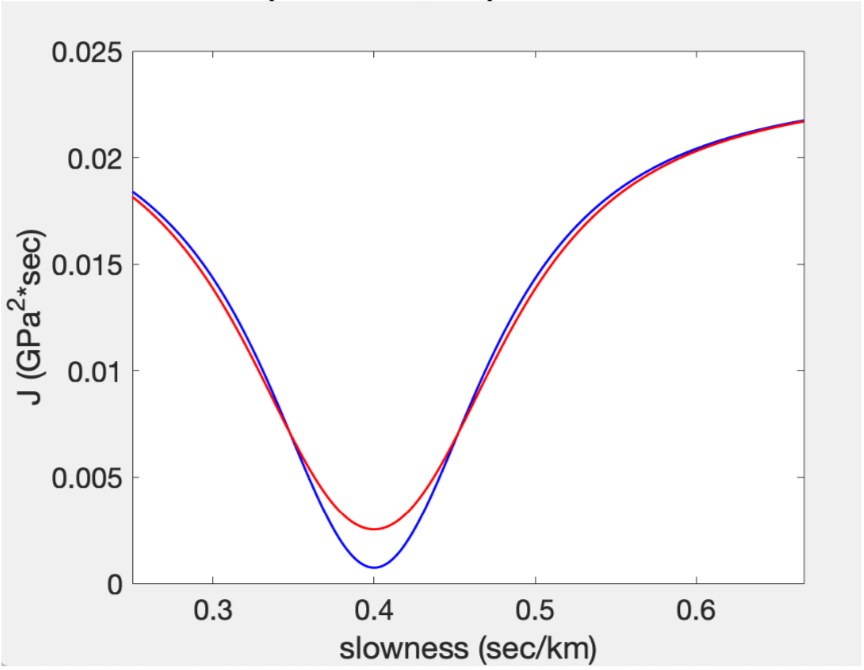
\includegraphics[height=5cm]{Fig/VPM.png}
\end{center}
\vspace{-0.5cm}
Red: $\lambda=0.05$ s (20 Hz), Blue: $\lambda = 0.025$ s (40 Hz) [H. Chen et al. SEG 20]
}
\only<5>{
$J_{\rm MSI} vs. J_{\rm FWI}$: $d=F[m_*]w_{\lambda}$, $m_*=0.4$ s/km, $w_{\lambda}$ = Ricker ctr freq = 40 Hz ($\lambda = 0.025$ s), $h=1$ km, $\alpha=1 s^{-1}km^{-1}$
\vspace{-0.5cm}
\begin{center}
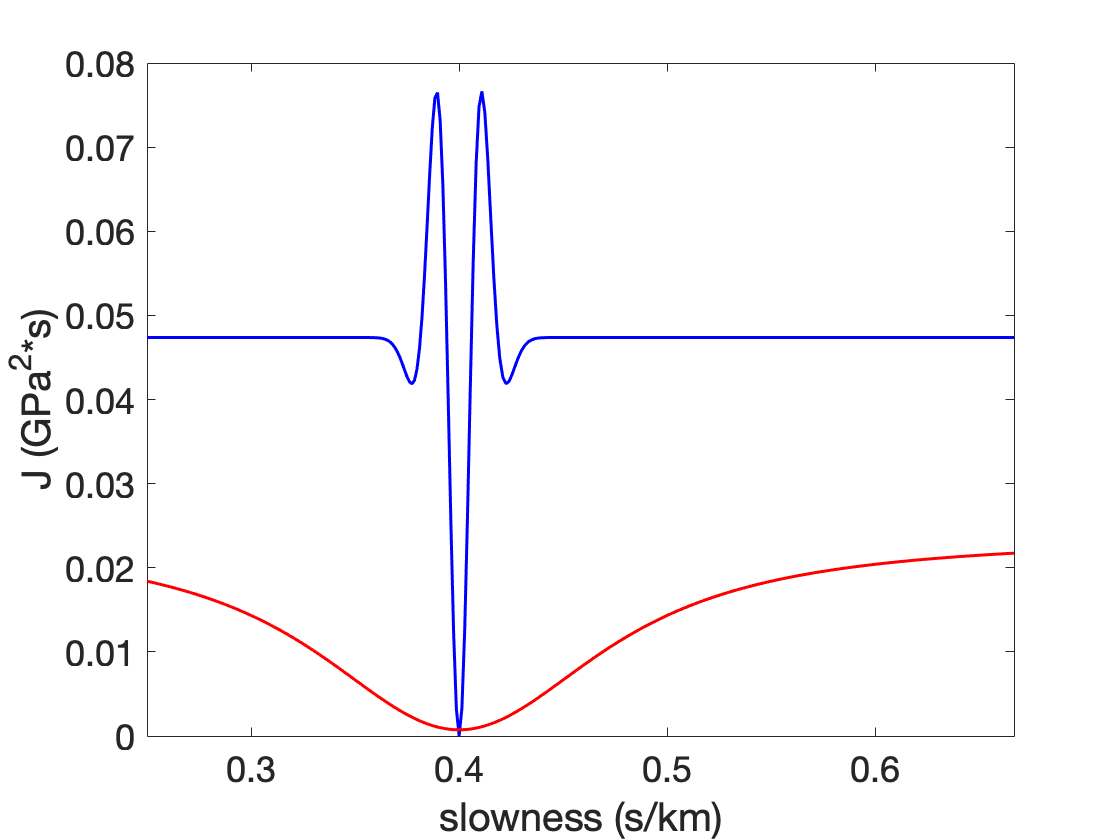
\includegraphics[height=5cm]{Fig/FWI-VPM-40.png}
\end{center}
\vspace{-0.5cm}
Red: MSI, Blue: FWI [H. Chen et al. SEG 20]
}
\only<6>{
$J_{\rm MSI} vs. J_{\rm FWI}$: $d=F[m_*]w_{\lambda}+n$, $n$ = 100\% RMS filtered stationary random noise, otherwise same
\vspace{-0.5cm}
\begin{center}
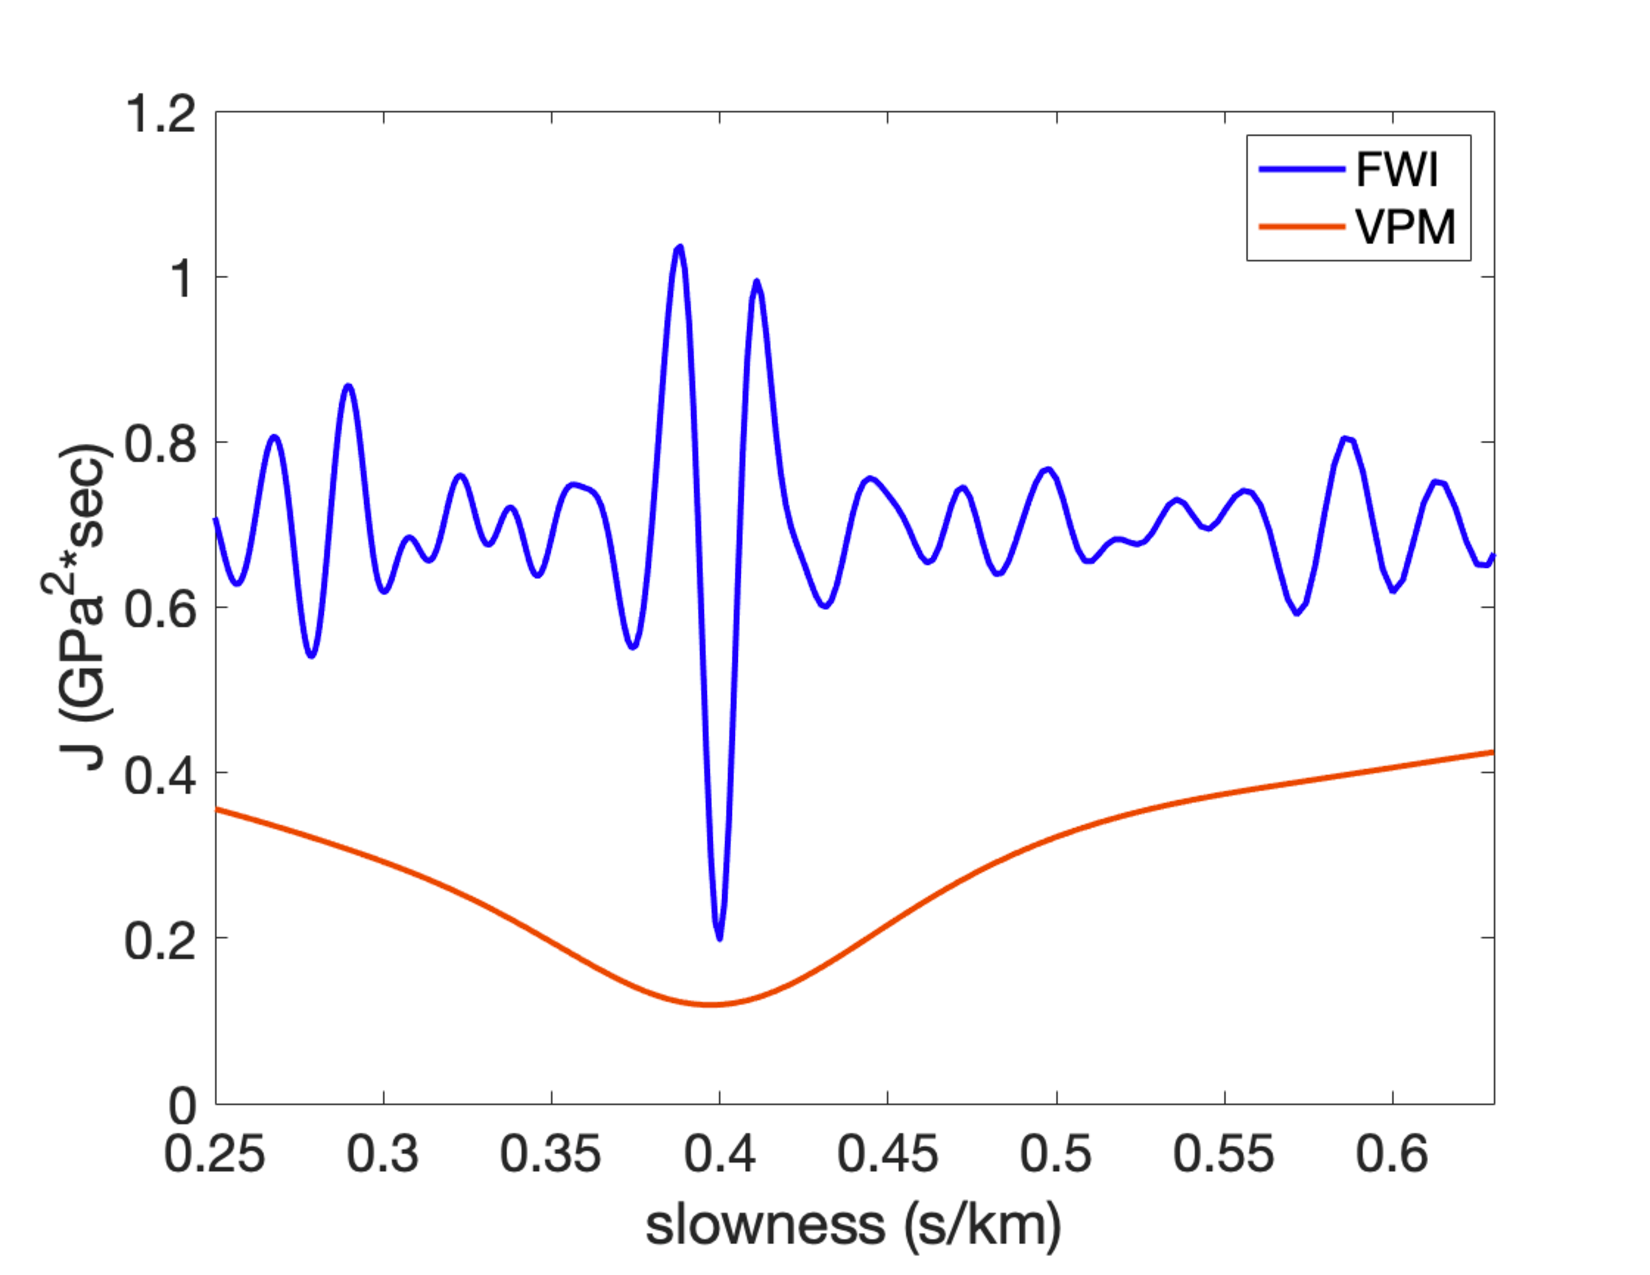
\includegraphics[height=5cm]{Fig/FWI-VPM-noisy.pdf}
\end{center}
\vspace{-0.5cm}
Red: MSI, Blue: FWI [H. Chen]
}
\only<7>{
Verdict: MSI
\begin{itemize}
\item appears to avoid cycle-skipping
\item ``hugs data'', expands search space - but effectively
\item Lots of multi-D relatives show good cycle-skip busting examples:  matched source extension (Huang \& S. 16), volume and space-time source extensions (Huang et al GEO 18), surface source extension (Huang et al. SEG 19), receiver shift extension (M\'{e}tivier SEG 20),  AWI (Warner \& Guatsch GEO 16 - field scale 3D, commercial)
\end{itemize}
}
\end{frame}

\begin{frame}\frametitle{So why?}
\only<1>{
Common penalty form for extended source inversion methods:
\[
\min_{m,w} \|F[m]w-d\|^2 + \alpha^2 \|Aw\|^2
\]
\begin{itemize}
\item $m = $ vector of parameter {\em fields} incl. velocities
\item $F[m] = $ modeling operator
\item $d=$ multichannel data 
\item $w$ =  extended source, $A = $ annihilator: physical source satisfy $Aw \approx 0$
\end{itemize}
Example: (AWI/MSI) point radiator  $w(t)\delta(\bx-\bx_s)$: physical source = impulsive, focused at $t=0$; extended source: spread in $t$; $Aw(t)=tw(t)$.
}
\only<2>{
Necessary condition: reduced objective (VPM) must be regular (differentiable) in $m, d$ {\em jointly}

For penalty functions as above: $A$ {\em must} be (pseudo)differential (Stolk \& S 03)

Re-write of FWI, WRI reduced objectives: analogous op {\em not} pseudodifferential

\begin{itemize}
\item FWI, WRI {\em fail}, MSI {\em passes} (S. IP 20)
\end{itemize}


}
\only<3>{
Sufficient condition: gradient related to traveltime tomography gradient
\begin{itemize}
\item Structure of wave-based modeling operators:
\[
D_m (F[m]w)\delta m = {\color{blue}Q[m,\delta m]}F[m]w
\]
$Q$ = order 1 approx. skew-symm. (pseudo)differential op
\end{itemize}
Example: (AWI/MSI) $F[m]w(\bx_r,t) \approx a(\bx_s,\bx_r)w(t-\tau[m](\bx_s,\bx_r))$, so
\[
D_m (F[m]w)\delta m \approx {\color{blue}-D\tau(\bx_s,\bx_r)\delta m\frac{\partial}{\partial t}}F[m]w
\] 
(chain rule!)
}
\only<4>{
(...bunch of algebra...) $\Rightarrow$ 
\[
\nabla J_{\rm MSI} \propto \nabla_m \|\tau[m]-\tau_{\rm data}\|^2
\]
so MSI $\approx$ travel time inversion

And that's why.

(Chen et al. SEG 20, Huang \& S. SEG 16) 
}
\end{frame}

\begin{frame}\frametitle{Thanks to...}
\begin{itemize}
\item Prof. Susan. E. Minkoff, GRA Huiyi Chen, UT Dallas
\item Guanghui Huang (PGS), Rami Nammour, Mohamed Dolliazal, Paul Williamson (Total)
\item many other students, postdocs, and colleagues
\item former sponsors of The Rice Inversion Project (1992-2019)
\item you!
\end{itemize}
\end{frame}

\begin{frame}\frametitle{Key References}
G. Huang et al., ``Waveform Inversion by Source Extension'': SEG 2019

H. Chen et al., ``Full waveform inversion by source extension: why it works", SEG 2020

W. Symes, ``Wavefield reconstruction inversion: an example'', {\em Inverse Problems} v. 36(10), 2020
\end{frame}



\end{document}


